\documentclass{article}
\usepackage[a4paper, total={6.5in, 9.6in}]{geometry}
\usepackage{multirow}
\usepackage{import}
\usepackage{graphicx}
\usepackage{listings}
\usepackage{color}
\usepackage{float}
\usepackage{amsmath}
%\usepackage{hyperref}
\usepackage{url}

\newcommand\Tstrut{\rule{0pt}{2.6ex}}         % = `top' strut
\newcommand\Bstrut{\rule[-0.9ex]{0pt}{0pt}}   % = `bottom' strut

\newcommand\todo[1]{\textit{\textcolor{mauve}{[TODO: #1]}}} % TODO Tag
\newcommand\emptyline{\vspace{\baselineskip}} % empty line

\definecolor{dkgreen}{rgb}{0,0.6,0}
\definecolor{gray}{rgb}{0.5,0.5,0.5}
\definecolor{mauve}{rgb}{0.58,0,0.82}

\lstset{frame=tb,
	language=Java,
	aboveskip=3mm,
	belowskip=3mm,
	showstringspaces=false,
	columns=flexible,
	basicstyle={\small\ttfamily},
	numbers=none,
	numberstyle=\tiny\color{gray},
	keywordstyle=\color{blue},
	commentstyle=\color{dkgreen},
	stringstyle=\color{mauve},
	breaklines=true,
	breakatwhitespace=true,
	tabsize=3
}

\begin{document}

\title{Text Classification using Naive Bayes}

\date{October 20, 2021}

\author{%
	Name: Lin Sun\\
	Email: lxs5171@mavs.uta.edu
}

\maketitle

\section*{Abstract}

Naive Bayes classifier might be the most popular and efficient classifier for text classification in the era of traditional machine learning, for its simplicity in concept and high performance. In this project, we step by step built a Naive Bayes classifier for a corpus with messages from 20 newsgroups. An optimal smoothing factor is selected by cross-validation, with which the overall average precision on these 20 categories can reach up to 88.5\% without any help of feature selection or any other methods. We also conducted simple noise-removing method and can see up to 17.6\% improvement of the precision performance for some categories, which indicating a large room for feature selection research in this area.

\section{Naive Bayes Classifier}
\label{sec:nb-classifier}

Naive Bayes Classifier is a very useful tool has a wide range application. It is a kind of generative classifier that performs supervised machine learning in comparison with the discriminative and unsupervised ones. It makes prediction according to the combination of prior probabilities. In the era of traditional machine learning, it could be the best classifier against several common classifiers (such as decision tree, neural network, and support vector machines) in term of accuracy and computational efficiency \cite{is-nb-good} when tuned carefully. Naive Bayes Classifier is derived from Bayes Rules \cite{bayes-rule} and constrained by an independence assumption:

\begin{itemize}
	\item \textbf{Bayes Rule} is a theorem in probability and statistics, describes the probability of an event based on prior knowledge of conditions that might be related to the event  \cite{bayes-rule}. 
	\begin{equation} \label{eq:bayes-rule}
		P(A|B)=\frac{P(B|A)P(A)}{P(B)}
	\end{equation}
	The equation \ref{eq:bayes-rule} of Bayes Rule indicates that we can make predictions according to certain properties of the event, if we extend event $B$ to a set of events $\{X_1, X_2, \ldots, X_n\}$ related to event $A$.
	\begin{equation} \label{eq:bayes-rule-extended}
		P(A_i|{X_1 \ldots X_n})=\frac{P(A_i)P(X_1...X_n|A_i)}{\sum_j{P(A_j)P(X_1...X_n|A_j)}}
	\end{equation}
	From equation \ref{eq:bayes-rule-extended} we can see the prediction of posterior probabilities can be transformed to the evaluation of a set prior probabilities. However, it's impractical for the unbiased learning of Bayes Classifier by counting every possible combination of the related events, because there would have $2(2^n-1)$ parameters to evaluate.
	\item \textbf{Independence Assumption} is necessary to reduce the evaluation space to only $2n$ parameters, where we assume every related event $X_i$ is conditionally independent of any other related event $X_j$ given any possible value of event $A$. With this assumption, we can represent the combination of related events $P(X_1 \ldots X_n|A)$ as $P(X_1|A)\cdot P(X_2|A) \cdots P(X_n|A)$. i.e.,
	\begin{equation} \label{eq:independence-product}
		P(X_1 \ldots X_n|A)=\prod_{i=1}^{n}{P(X_i|A)}
	\end{equation}
	Then, the equation of Bayes Rule can be simplified to:
	\begin{equation} \label{eq:naive-bayes}
		P(A_i|{X_1 \ldots X_n})=\frac{P(A_i)\prod_{k}{P(X_k|A_i)}}{\sum_j{P(A_j)\prod_{k}{P(X_k|A_j)}}}
	\end{equation}
	And for every possible value $A_i$ the denominator is the same, so to predict which $A_i$ is the most possible value, is to estimate the maximum likelihood of $A$:
	\begin{equation} \label{eq:naive-bayes}
		A \leftarrow \arg\max_{j} {P(A_j)\prod_{i}{P(X_i|A_j)}}
	\end{equation}
	Therefore, we can simplify the parameter evaluation and only use the conditional probabilities of individually related event instead of their combinations. However, we need to keep in mind of the assumption which is the basis of Naive Bayes, and try to minimize the conditional dependence between the related events.
\end{itemize}

\section{Text Classification}

Text classification is an important topic among traditional Text Retrieval \cite{trec}, which is a branch of Natural Language Processing (NLP) \cite{chowdhury2003natural}. It's to classify each document into pre-learned classes, usually by the Bag-of-words feature model \cite{bag-of-words} or/and semantic model \cite{semantic-text-classification} using Ontology \cite{ontology-learning}. When there are only two classes it becomes a filtering task, e.g., filter out spam emails from incoming message streams. As figure \ref{fig:text-classification} shown, a typical text classification system is usually layered into three layers \cite{document-cleaning}. The learning and classification modules on the top and share the underlying layers, by which the original documents (usually semi-structured or unstructured) in the corpus are transformed to structured representations. 

\begin{figure}[!ht]
	\centering
	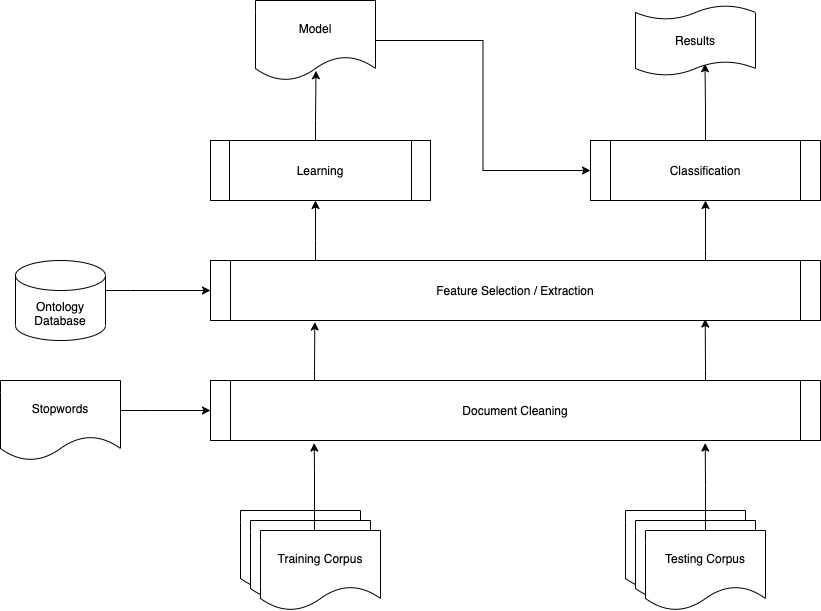
\includegraphics[scale=0.45]{img/text-classification.jpg}
	\caption{Typical Text Classification system}
	\label{fig:text-classification}
\end{figure}

\begin{itemize}
	\item the \textit{Document Cleaning} layer \cite{document-cleaning} is to parse the document into "bag-of-words" and try to eliminate obvious noises, such as bad format, words containing characters in unrecognizable codes, case sensitivity, hyphens, and so on.
	\item the \textit{Feature Selection} layer, also known as \textit{Feature Extraction}, is to transform the "bag-of-words" into features \cite{feature-selection-and-extraction}. This is a critical step for text classification which could dramatically influence the performance of learning and classification. For example, as evaluated in TREC2005, when domain-specific features are selected for biomedical articles, the classification performance outperformed its contemporary competitors a lot \cite{wim2005}. The ontology based and other kinds of semantic analysis can be applied here to improve feature quality \cite{vicient2013automatic, wang2003comparative}.
\end{itemize}

\section{Text Classification using Naive Bayes Classifier}

Naive Bayes could be the most popular classifier for text classification \cite{kim2006some, mccallum1998comparison, chen2009feature, dai2007transferring}, for its simplicity in concept and high performance in both accuracy and efficiency \cite{is-nb-good}. As discussed in section \ref{sec:nb-classifier}, in order to use Naive Bayes classifier, the prediction needs to be made according to a collection of related events. In other words, the features of each samples are considered as related events of whether a sample belongs to a class or not. When applied in text classification, we need to evaluate the probability of each feature (known as \textbf{term}, or word) related with each class. And according to the independence assumption, it's better to make all the features conditional independent with each other, given the classes. 

\subsection{Learning: Parameter Evaluation}

Basically there are three ways to evaluate the probability for each term against each class, using Maximum Likelihood Estimation (MLE) 
\begin{itemize}
	\item \textbf{Binary}: whether a term appears in a class of documents. No matter how many times it appears, only count once.
	\begin{equation}\label{eq:binary}
		P_{ij}^{b}=P(term_i|class_j)_{binary}=\begin{cases}
				1, & \text{if $term_i$ appears in any documents of $class_j$}  \\
				0, & \text{if $term_i$ does not appear in $class_j$}
		\end{cases}
	\end{equation}
	\item \textbf{Document Frequency}: how many documents a term appears in a class. Specifically, 
	\begin{equation}\label{eq:df}
		P_{ij}^{df}=P(term_i|class_j)_{df}=\frac{\#D\{\text{documents contain $term_i$ in $class_j$}\}}{\#D\{\text{documents in $class_j$}\}}
	\end{equation}
	\item \textbf{Term Frequency}: how many times a term appears in all the documents of a class, i.e., regarding all the documents in a class as a single document:
	\begin{equation}\label{eq:tf}
		P_{ij}^{tf}=P(term_i|class_j)_{tf}=\frac{\#W\{\text{$term_i$ in $class_j$}\}}{\#W\{\text{all terms in $class_j$}\}}
	\end{equation}
\end{itemize}

We can easily see equation \ref{eq:binary} and equation \ref{eq:tf} are two extreme cases of calculating the conditional probability. A good model usually comes from somewhere between them. Essentially, equation \ref{eq:tf} can be derived from equation \ref{eq:df} multiply the ratio weight of the $term_i$:

\begin{equation} \label{eq:tf-df}
	P_{ij}^{tf}=P_{ij}^{df} \times \frac{\text{average of $term_i$ in $class_j$ documents that contains it}}{\text{average of terms in all documents of $class_j$}}  
\end{equation}

And equation \ref{eq:df} and equation \ref{eq:tf} are the Maximum Likelihood Estimation of the conditional probability of each $term_i$ in $class_j$. However, it would be totally different for the prior probability of each class when applying these two MLE equations. 

\begin{itemize}
	\item \textbf{Prior probability of each class when using document frequence} should count for the document number among the corpus
	\begin{equation}\label{eq:prior_df}
		P_{A=j}^{df}=\frac{\#D\{\text{documents in $class_j$}\}}{\#D\{\text{documents in the corpus}\}}
	\end{equation}
	\item \textbf{Prior probability of each class when using term frequence} should count for the amount of terms in each class among the corpus
	\begin{equation}\label{eq:prior_tf}
		P_{A=j}^{tf}=\frac{\#W\{\text{terms in $class_j$}\}}{\#W\{\text{terms in the corpus}\}}
	\end{equation}
\end{itemize}

\subsection{Prediction}

After representing an test sample as a set of terms. The classifier is to estimate the most possible class using the prior conditional probabilities of each term and class:

\begin{equation} \label{eq:naive-bayes-text-classification}
	class \leftarrow \arg\max_{j} {P(class_j)\prod_{i}{P(term_i|class_j)}}
\end{equation}

Where the conditional probability $P(term_k|class_i)$ comes from the results of parameter evaluation. As aforementioned, when applying \textit{document frequency} or \textit{term frequency}, the prior probability of each class $P(class_i)$ should change accordingly.

However, when performing prediction based very large dimension feature space, the product of $P(class_i)\prod_{k}{P(term_k|class_i)}$ could be too small to have any difference against each other. Instead, $log$ function is usually introduced to get comparable results which is equivalent for the MLE equation \ref{eq:naive-bayes-text-classification}:

\begin{equation} \label{eq:naive-bayes-text-classification-using-log}
	class \leftarrow \arg\max_{j} {\; \log(P(class_j)) + \sum_{i}{\log{(P(term_i|class_j))}}}
\end{equation}

\section{Naive Bayes Classification on 20 Categories Newsgroup}

The \textit{20 Categories Newsgroup} corpus \cite{corpus} contain around 20,000 newsgroup messages drawn from 20 newsgroups, as table \ref{table:corpus-dist} shown,  each of which contain around 1,000 messages.

\begin{table}[!ht]
	\centering
	\begin{tabular}{ |c|c| }
		\hline
		\textbf{Class} & \textbf{Amount of messages}\\
		\hline
		Italk.politics.mideast & 1,000 \\
		\hline
	    rec.autos & 1,000 \\
		\hline
		comp.sys.mac.hardware & 1,000 \\
		\hline
		alt.atheism & 1,000 \\
		\hline
		rec.sport.baseball & 1,000 \\
		\hline
		comp.os.ms-windows.misc & 1,000 \\
		\hline
		rec.sport.hockey & 1,000 \\
		\hline
		sci.crypt & 1,000 \\
		\hline
		sci.med & 1,000 \\
		\hline
		talk.politics.misc & 1,000 \\
		\hline
		rec.motorcycles & 1,000 \\
		\hline
		comp.windows.x & 1,000 \\
		\hline
		comp.graphics & 1,000 \\
		\hline
		comp.sys.ibm.pc.hardware & 1,000 \\
		\hline
		sci.electronics & 1,000 \\
		\hline
		talk.politics.guns & 1,000 \\
		\hline
		sci.space & 1,000 \\
		\hline
		soc.religion.christian & 997 \\
		\hline
		misc.forsale & 1,000 \\
		\hline
		talk.religion.misc & 1,000 \\
		\hline
	\end{tabular}
	\caption{Corpus sample distribution}
	\label{table:corpus-dist}
\end{table}

According to the architecture illustrated in figure \ref{fig:text-classification}, we build a text classification system using Naive Bayes classifier. Common stopwords list \cite{stopwords-list} is introduced to improve the quality of features. After \textit{document cleaning} and removing the stopwords, each single word is regard as a feature which is usually called as \textbf{term} in NLP. Although there are plenty of method to improve feature quality, here we adopt this most simple and intuitive way because the objective of this project is to evaluate the performance of \textit{Naive Bayes Classifier}. We even would not bother to use large dimension feature space directly without any reduction. 

During the learning phase, the prior conditional probability of each term is evaluated using aforementioned equations, and then stored in a matrix that we call it as \textit{Prior Probability Matrix} mark as \textbf{PPM}:

\begin{equation} \label{eq:ppm}
	PPM = \big[  x_{ij}  \big]
\end{equation}
 where $i$ is the \textit{ith} term among all distinct terms in the entire corpus, $j$ is the \textit{jth} class. The shape of PPM is $(\#\{classes\} \times \#\{terms in the corpus\} )$

Then for the prediction, we apply equation \ref{eq:naive-bayes-text-classification-using-log} for each test document. However, there is a problem when applying this equation directly. For any new words in the test document that appeared in the corpus but not appeared in the training set for a particular class, their conditional probabilities are zero, which is illegal for $log$ calculation and would make zero prediction if applying equation \ref{eq:naive-bayes-text-classification} directly by multiply the conditional probability of each term that appears in the test document.

To solve this problem, a \textbf{smoothing factor} is introduced for \textit{parameter evaluation}:

\begin{equation} \label{eq:smooth-factor}
	P_{ij}^{df}=P(term_i|class_j)_{df}=\frac
	{\#D\{\text{documents contain $term_i$ in $class_j$}\} + l }
	{\#D\{\text{documents in $class_j$}\} + lJ}
\end{equation}
where $l$ is the \textit{smoothing factor} which usually takes a value in the range of $(0, \; 1]$, and $J$ is the possible values that \textit{whether a document contains $term_i$} which obviously is $J=2$. And the equation \ref{eq:smooth-factor} corresponds to \textit{MAP} estimation. When $l=1$ it is called \textit{Laplace smoothing}, and when $l=0$ it is degenerating to the \textit{MLE} estimation which is identical with equation \ref{eq:df}. And it is the same if we are going to adopt \textit{term frequency} using equation \ref{eq:tf}.

Since there is a undecided parameter in the evaluation, i.e., the \textit{smoothing factor} $l$, it is natural to use \textit{Cross Validation} to select an optimal value.

\section{Cross Validation by Rolling}

Cross Validation is a useful tool to evaluate the performance of a model, especially useful for comparing different models or different settings of a model \cite{cross-validation}. In general, it is leveraging disjoint subsets of the randomly shuffled sample set to in turn evaluate the precision, and output an overall score upon all these subsets. There are many strategies when applying cross-validation, which mostly by changing the amount and combination of subsets for testing and using the rest for training during each time of evaluation. 

\subsection{Corpus separation}
However, in this project we are required to use half of the corpus for training and the other half for testing, i.e., 

\begin{equation} \label{eq:training-ratio}
	ratio_{test/training} = \frac{\#\{\text{samples for testing}\}}{\#\{\text{samples for training}\}} = 1
\end{equation}

So, we designed a cross-validation method by rolling across each samples in the class. For each round of training and testing, we split the corpus using a window rolling by a shift:

\begin{equation} \label{eq:roll-samples}
	sample_i \; \text{belongs to} \begin{cases}
		\text{training set, if $((i + s)\mod \;\; w)< \frac{1}{2} w $}  \\
		\text{testing set, otherwise}
	\end{cases}
\end{equation}
where $w$ is the \textit{window size} and $s$ is the \textit{shift} for each round. In the project, we set $w=10$. So, for each round of evaluation there would be $\frac{1}{10}$ different samples in the training set and testing set.

\subsection{Performance Evaluation}
For each round of evaluation, we calculate the \textit{MSE (Mean Square Error)} as the performance index:
\begin{equation} \label{eq:mse}
	MSE = \frac{\sum_j {(1-\text{precision}_j)^2}}{\#\{classes\}} 
\end{equation}
where,
\begin{equation} \label{eq:precision}
	precision_j = \frac{\# \{\text{correctly classified samples in $class_j$} \} }{\#\{\text{samples in $class_j$}\}} 
\end{equation}

After rolling over the corpus, the mean of MSEs for different rounds is used as the performance index for a particular parameter value, i.e., the smoothing factor. Then, the value with minimum $\text{perf}_{\text{smooth factor}} = \frac{\sum{MSE_s}}{\#\{\text{rounds of rolling}\}} $ is selected as the optimal value of the smoothing factor.

\begin{table}[!ht]
	\centering
	\begin{tabular}{ |c|c|c|c|c|c|c|c|c|c|c|c| }
		\hline
		\textbf{f} & \textbf{avg} & shift 0 & shift 1& shift 2& shift 3& shift 4& shift 5& shift 6& shift 7& shift 8& shift 9 \\
		\hline

0.1 & 0.025 & 0.023 & 0.022 & 0.022 & 0.023 & 0.024 & 0.026 & 0.028 & 0.027 & 0.029 & 0.026 \\
\hline
0.2 & 0.026 & 0.024 & 0.023 & 0.023 & 0.023 & 0.025 & 0.028 & 0.029 & 0.028 & 0.029 & 0.027 \\
\hline
0.3 & 0.027 & 0.025 & 0.024 & 0.023 & 0.024 & 0.026 & 0.029 & 0.03 & 0.028 & 0.03 & 0.028 \\
\hline
0.4 & 0.028 & 0.026 & 0.025 & 0.024 & 0.025 & 0.026 & 0.029 & 0.031 & 0.029 & 0.031 & 0.029 \\
\hline
0.5 & 0.028 & 0.027 & 0.025 & 0.025 & 0.025 & 0.027 & 0.03 & 0.032 & 0.029 & 0.032 & 0.029 \\
\hline
0.6 & 0.029 & 0.027 & 0.026 & 0.025 & 0.026 & 0.027 & 0.03 & 0.032 & 0.03 & 0.033 & 0.03 \\
\hline
0.7 & 0.029 & 0.028 & 0.026 & 0.026 & 0.027 & 0.027 & 0.031 & 0.033 & 0.03 & 0.033 & 0.03 \\
\hline
0.8 & 0.03 & 0.029 & 0.027 & 0.027 & 0.027 & 0.028 & 0.031 & 0.034 & 0.031 & 0.034 & 0.031 \\
\hline
0.9 & 0.03 & 0.029 & 0.027 & 0.027 & 0.028 & 0.028 & 0.031 & 0.034 & 0.032 & 0.034 & 0.031 \\
\hline
1.0 & 0.031 & 0.03 & 0.028 & 0.028 & 0.029 & 0.029 & 0.032 & 0.035 & 0.033 & 0.035 & 0.032 \\
\hline

\end{tabular}
\caption{MSE score of Cross Validation by Rolling}
\label{table:result-cv}
\end{table}

\section{Feature Selection}

The only feature selection method we applied is the \textit{stopwords}. And the raw words are used directly as features with minimum document cleaning, that only trimmed words to eliminate special characters on both sides of each word, and turned words into lower cases to uniform each term.

The feature space is sparse. Table \ref{table:feature-dist} shows the feature space distribution for the training set with $\text{shift}=0$ as an example. Each category only occupies a little portion with the overall feature space, which varies from 6.8\% to 12.9\%. What for sure is, the sparse feature space with hundreds of thousands of features, introduces large of computation difficulties in precision and efficiency, while Naive Bayes classifier is able to doing well on both of them.

\begin{table}[!ht]
	\centering
	\begin{tabular}{ |c|c|c| }
		\hline
		\textbf{class} & \textbf{terms} & \textbf{portion} \\
		\hline
		\textbf{overall} & 171,422 & 100\% \\
		\hline
		Italk.politics.mideast & 20,222 & 11.8\%\\
		\hline
		rec.autos & 13,352 & 7.8\% \\
		\hline
		comp.sys.mac.hardware & 11,723 & 6.8\% \\
		\hline
		alt.atheism & 13,276 & 7.7\%  \\
		\hline
		rec.sport.baseball & 12,832 & 7.5\% \\
		\hline
		comp.os.ms-windows.misc & 22,054 & 12.9\% \\
		\hline
		rec.sport.hockey & 16,275 & 9.5\% \\
		\hline
		sci.crypt & 16,706 & 9.7\% \\
		\hline
		sci.med & 18,053 & 10.5\% \\
		\hline
		talk.politics.misc & 18,624 & 10.9\% \\
		\hline
		rec.motorcycles & 13,145 & 7.7\% \\
		\hline
		comp.windows.x & 19,428 & 11.3\% \\
		\hline
		comp.graphics & 17,430 & 10.2\% \\
		\hline
		comp.sys.ibm.pc.hardware & 12,477 & 7.3\% \\
		\hline
		sci.electronics & 13,327 & 7.8\% \\
		\hline
		talk.politics.guns & 16,476 & 9.6\% \\
		\hline
		sci.space & 16,324 & 9.5\% \\
		\hline
		soc.religion.christian & 15,322 & 8.9\% \\
		\hline
		misc.forsale & 13,605 & 7.9\% \\
		\hline
		talk.religion.misc & 16,937 & 9.9\% \\
		\hline
	\end{tabular}
	\caption{Feature space distribution}
	\label{table:feature-dist}
\end{table}

However,  whether the portion a category takes is small or big, does not necessarily lead to poor or good precision performance. Let's take the categories with highest and lowest precision as an example, as table \ref{table:feature-perf} shows, the portion they take in the feature space is similar to each other, and both are close to the average level. 

\begin{table}[!ht]
	\centering
	\begin{tabular}{ |c|c|c| }
		\hline
		\textbf{class} & \textbf{precision} & \textbf{portion} \\
		\hline
		soc.religion.christian & 0.993 & 8.9\% \\
		\hline
		talk.religion.misc & 0.542 & 9.9\% \\
		\hline
		
	\end{tabular}
	\caption{Feature space vs precision performance}
	\label{table:feature-perf}
\end{table}

\section{Results}

To simplify the model and to focus on the performance of the classifier, we only adopt the parameter evaluation method of \textit{document frequency}. A set of cross-validation is applied against the smoothing factor in the range of $[0.1, 1.0]$. As table \ref{table:result-cv} shown, the optimal value of smoothing factor is $0.1$ which comes out with the minimum average MSE score.

Then, we use the optimal smoothing factor to train on the corpus using half of the samples and to test with the other half. In the end, we take the average precision as the performance index for each class by the aforementioned cross-validation method. As table \ref{table:result-precisions} shows, the precision performance for these 20 classes varies from 54.2\% for the class \textit{talk.religion.misc} to 99.3\% for the class \textit{soc.religion.christian}. The overall precision for all these 20 classes is 88.5\%.

We also find a phenomenon that the lowest precision class \textit{talk.religion.misc} is usually the biggest error source for other classes. Once it is removed from the corpus, as table \ref{table:result-noise-removing} shows, the performance for some other classes can be improved greatly. For the class \textit{alt.atheism}, its precision improved from 77.7\% to 91.4\% with 17.6\% improvement. This may indicates some degrees of correlation between these two classes regarding the selected terms. As we know, the Naive Bayes classifier assumes conditional independent for the features. So, the simple result of table \ref{table:result-noise-removing} intuitively indicates that the performance of Naive Bayes classifier can be improved greatly by sophisticated feature selection, and particularly, there is a large room for domain-specific feature selection research in this area.

\begin{table}[!ht]
	\centering
	\begin{tabular}{ |c|c|c|c|c|c|c|c|c|c|c|c| }
		\hline
		\textbf{class} & \textbf{avg} & shift 0 & 1& 2& 3& 4& 5& 6& 7& 8& 9 \\
		\hline

alt.atheism & 0.777  & 0.71 & 0.72 & 0.79 & 0.82 & 0.81 & 0.84 & 0.83 & 0.74 & 0.74 & 0.76 \\
\hline
comp.graphics & 0.883  & 0.94 & 0.91 & 0.91 & 0.89 & 0.84 & 0.83 & 0.84 & 0.86 & 0.88 & 0.92 \\
\hline
comp.os.ms-windows.misc & 0.844  & 0.82 & 0.84 & 0.83 & 0.86 & 0.87 & 0.87 & 0.86 & 0.85 & 0.83 & 0.8 \\
\hline
comp.sys.ibm.pc.hardware & 0.866  & 0.86 & 0.87 & 0.84 & 0.83 & 0.82 & 0.85 & 0.88 & 0.9 & 0.91 & 0.9 \\
\hline
comp.sys.mac.hardware & 0.899  & 0.89 & 0.9 & 0.93 & 0.93 & 0.91 & 0.9 & 0.92 & 0.86 & 0.88 & 0.87 \\
\hline
comp.windows.x & 0.936  & 0.92 & 0.93 & 0.93 & 0.95 & 0.94 & 0.95 & 0.96 & 0.95 & 0.92 & 0.92 \\
\hline
misc.forsale & 0.731  & 0.75 & 0.75 & 0.74 & 0.72 & 0.71 & 0.71 & 0.71 & 0.75 & 0.73 & 0.74 \\
\hline
rec.autos & 0.915  & 0.9 & 0.92 & 0.93 & 0.92 & 0.92 & 0.9 & 0.92 & 0.91 & 0.91 & 0.92 \\
\hline
rec.motorcycles & 0.953  & 0.95 & 0.94 & 0.94 & 0.95 & 0.95 & 0.95 & 0.98 & 0.96 & 0.96 & 0.96 \\
\hline
rec.sport.baseball & 0.964  & 0.96 & 0.96 & 0.97 & 0.97 & 0.97 & 0.97 & 0.97 & 0.96 & 0.97 & 0.96 \\
\hline
rec.sport.hockey & 0.981  & 0.98 & 0.98 & 0.97 & 0.97 & 0.97 & 0.98 & 0.98 & 0.99 & 0.99 & 0.99 \\
\hline
sci.crypt & 0.975  & 0.96 & 0.98 & 0.98 & 0.99 & 0.99 & 0.98 & 0.98 & 0.98 & 0.96 & 0.95 \\
\hline
sci.electronics & 0.869  & 0.87 & 0.87 & 0.83 & 0.83 & 0.86 & 0.86 & 0.88 & 0.9 & 0.88 & 0.91 \\
\hline
sci.med & 0.939  & 0.96 & 0.95 & 0.93 & 0.93 & 0.94 & 0.92 & 0.93 & 0.94 & 0.94 & 0.94 \\
\hline
sci.space & 0.957  & 0.94 & 0.96 & 0.96 & 0.95 & 0.97 & 0.97 & 0.96 & 0.95 & 0.96 & 0.95 \\
\hline
soc.religion.christian & 0.993  & 0.99 & 0.99 & 1.0 & 0.99 & 0.99 & 0.98 & 1.0 & 1.0 & 1.0 & 0.99 \\
\hline
talk.politics.guns & 0.898  & 0.9 & 0.91 & 0.9 & 0.87 & 0.89 & 0.89 & 0.89 & 0.89 & 0.92 & 0.91 \\
\hline
talk.politics.mideast & 0.975  & 0.97 & 0.97 & 0.96 & 0.96 & 0.98 & 0.98 & 0.98 & 0.98 & 0.98 & 0.98 \\
\hline
talk.politics.misc & 0.799  & 0.79 & 0.77 & 0.8 & 0.79 & 0.78 & 0.8 & 0.81 & 0.82 & 0.81 & 0.81 \\
\hline
talk.religion.misc & 0.542  & 0.61 & 0.63 & 0.59 & 0.58 & 0.58 & 0.52 & 0.45 & 0.49 & 0.47 & 0.51 \\
\hline

\end{tabular}
\caption{Precisions of each class with the optimal smoothing factor 0.1}
\label{table:result-precisions}
\end{table}

\begin{table}[!ht]
	\centering
	\begin{tabular}{ |c|c|c| }
		\hline
		\textbf{class} & \textbf{after} & \textbf{before} \\
		\hline
		
		alt.atheism & 0.914  & 0.777 \\
		\hline
		comp.graphics & 0.91 & 0.883   \\
		\hline
		comp.os.ms-windows.misc & 0.84 & 0.844  \\
		\hline
		comp.sys.ibm.pc.hardware & 0.872 & 0.866  \\
		\hline
		comp.sys.mac.hardware & 0.904 & 0.899 \\
		\hline
		comp.windows.x & 0.932 & 0.936 \\
		\hline
		misc.forsale & 0.752 & 0.731  \\
		\hline
		rec.autos & 0.926 & 0.915  \\
		\hline
		rec.motorcycles & 0.938 & 0.953  \\
		\hline
		rec.sport.baseball & 0.956 & 0.964 \\
		\hline
		rec.sport.hockey & 0.976 & 0.981  \\
		\hline
		sci.crypt & 0.98 & 0.975 \\
		\hline
		sci.electronics & 0.87 & 0.869  \\
		\hline
		sci.med & 0.954 & 0.939 \\
		\hline
		sci.space & 0.964 & 0.957  \\
		\hline
		soc.religion.christian & 0.992 & 0.993  \\
		\hline
		talk.politics.guns & 0.936 & 0.898  \\
		\hline
		talk.politics.mideast  & 0.974 & 0.975  \\
		\hline
		talk.politics.misc & 0.852 & 0.799  \\
		\hline
		
	\end{tabular}
	\caption{Comparison of precision before and after noise removing}
	\label{table:result-noise-removing}
\end{table}

\newpage
\bibliographystyle{plainurl}
\bibliography{bibliography}


\end{document}
